\documentclass{article}%
\usepackage[T1]{fontenc}%
\usepackage[utf8]{inputenc}%
\usepackage{lmodern}%
\usepackage{textcomp}%
\usepackage{lastpage}%
\usepackage{geometry}%
\geometry{margin=1in,headheight=14pt,headsep=25pt}%
\usepackage{hyperref}%
\usepackage{enumitem}%
\usepackage{fancyhdr}%
\usepackage{xcolor}%
\usepackage{url}%
\usepackage{breakurl}%
\usepackage{amsmath}%
\usepackage{amssymb}%
\usepackage{mathtools}%
\usepackage{amsthm}%
\usepackage{thmtools}%
\usepackage{float}%
\usepackage{subcaption}%
\usepackage[font=small,labelfont=bf]{caption}%
%

            \hypersetup{
                colorlinks=true,
                linkcolor=blue,
                filecolor=magenta,
                urlcolor=blue,
                breaklinks=true,
                bookmarks=true,
                pdfborder={0 0 0}
            }
            \urlstyle{same}
            \Urlmuskip=0mu plus 1mu  % URL breaking in nicer spots

            % Math configuration
            \everymath{\displaystyle}
            \setlength{\jot}{10pt}  % Increase spacing between equations

            \pagestyle{fancy}
            \fancyhf{}
            \rhead{Generated on \today}
            \cfoot{\thepage}

            % Better Unicode support
            \usepackage[utf8]{inputenc}
            \usepackage{newunicodechar}
            \setlength{\itemsep}{1em} % Adds spacing between items

            % Configure itemize settings globally
            \setlist[itemize]{nosep}
            \setlist[itemize]{leftmargin=*}

            % Remove section numbering
            \renewcommand{\thesection}{}
            \renewcommand{\thesubsection}{}

            % Adjust caption spacing around figures
            \setlength{\abovecaptionskip}{0pt}
            \setlength{\belowcaptionskip}{5pt}
        %
\lhead{Lecture: 09L1{-}cnn}%
\title{09L1{-}cnn}%
\author{Generated by Scribe.AI}%
\date{\today}%
%
\begin{document}%
\normalsize%
\maketitle%
\section{Slide 1}%
\label{sec:Slide1}%
\subsection{Content}%

\textbf{CS 24300 - AI Basics}

\textbf{Tony Bergstrom}

\textbf{Slides adapted from Yexiang Xue}
%
\subsection{Description}%
This slide is a title slide for a lecture on Artificial Intelligence Basics, likely part of a course called CS 24300.  It displays the course title, the instructor's name (Tony Bergstrom), and a credit line indicating that the slides are adapted from another source (Yexiang Xue).  The background is a dark gray, and the text is light gray, making it easily readable.  The overall presentation is simple and professional, typical of a lecture slide layout.%
\subsection{Figures}%
\begin{figure}[H]%
\centering%
\end{figure}

%
\newpage%
\section{Slide 2}%
\label{sec:Slide2}%
\subsection{Content}%

\textbf{Convolutional Neural Network} \\
\textbf{for Image/Video Recognition}
%
\subsection{Description}%
This slide, likely part of a lecture on Artificial Intelligence Basics, introduces the topic of Convolutional Neural Networks (CNNs) for image and video recognition.  The title is displayed prominently.  The slide likely contains images illustrating the application of CNNs to various tasks.  The images shown are examples of image recognition tasks, including:  (1) face recognition (multiple views of a face with labeled points), (2) autonomous driving (lane detection and vehicle recognition), (3) object detection (detecting objects like a TV, cat, and fruit in a scene), and (4) potentially a digit recognition task (a grid of handwritten digits).  The context of the course is focused on the use of CNNs as a powerful technique in image and video analysis within the broader field of AI.%
\subsection{Figures}%
\begin{figure}[H]%
\centering%
\begin{subfigure}[b]{0.15\textwidth}%
\centering%

\includegraphics[width=\textwidth]{/Users/ashoksaravanan/Coding/ScribeLec/server/output/CS 243/lectures/09L1-cnn/figures/2.1.png}%
\caption{}%
\end{subfigure}%
\hspace{0.05\textwidth}%
\begin{subfigure}[b]{0.15\textwidth}%
\centering%

\includegraphics[width=\textwidth]{/Users/ashoksaravanan/Coding/ScribeLec/server/output/CS 243/lectures/09L1-cnn/figures/2.2.png}%
\caption{}%
\end{subfigure}%
\hspace{0.05\textwidth}%
\begin{subfigure}[b]{0.15\textwidth}%
\centering%

\includegraphics[width=\textwidth]{/Users/ashoksaravanan/Coding/ScribeLec/server/output/CS 243/lectures/09L1-cnn/figures/2.3.png}%
\caption{}%
\end{subfigure}%
\hspace{0.05\textwidth}%
\begin{subfigure}[b]{0.15\textwidth}%
\centering%

\includegraphics[width=\textwidth]{/Users/ashoksaravanan/Coding/ScribeLec/server/output/CS 243/lectures/09L1-cnn/figures/2.4.png}%
\caption{}%
\end{subfigure}%
\end{figure}

%
\newpage%
\section{Slide 3}%
\label{sec:Slide3}%
\subsection{Content}%

\textbf{ImageNet Top-5 Classification Accuracy} \\
15 million images 1000 classes in the ImageNet challenge \\
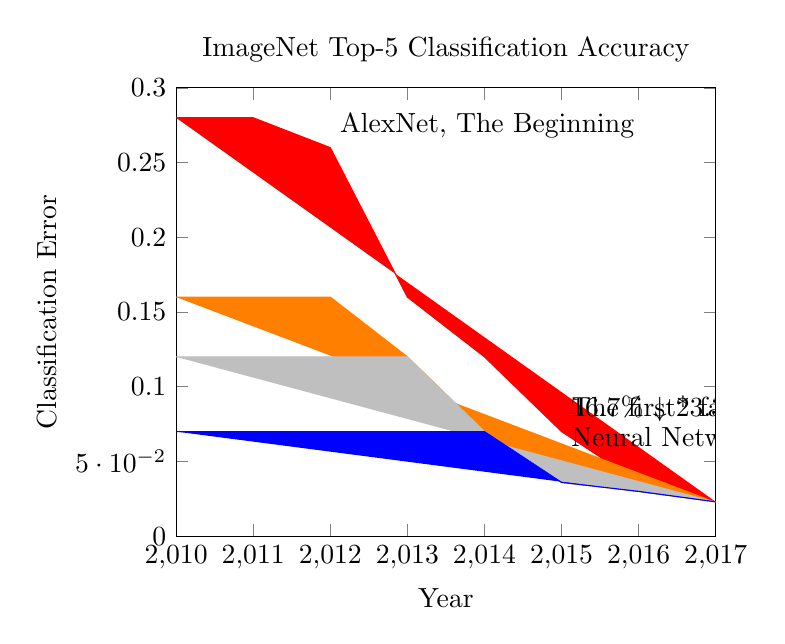
\begin{tikzpicture}
\begin{axis}[
    xlabel={Year},
    ylabel={Classification Error},
    xmin=2010, xmax=2017,
    ymin=0, ymax=0.3,
    xtick={2010,2011,2012,2013,2014,2015,2016,2017},
    ytick={0,0.05,0.1,0.15,0.2,0.25,0.3},
    title={ImageNet Top-5 Classification Accuracy},
    legend pos=north east,
]
\addplot[
    color=red,
    fill=red,
    area legend
]
coordinates {(2010,0.28) (2011,0.28) (2012,0.26) (2013,0.16) (2014,0.12) (2015,0.07) (2016,0.036) (2017,0.023)};
\addplot[
    color=orange,
    fill=orange,
    area legend
]
coordinates {(2010,0.16) (2011,0.16) (2012,0.16) (2013,0.12) (2014,0.07) (2015,0.036) (2016,0.03) (2017,0.023)};
\addplot[
    color=lightgray,
    fill=lightgray,
    area legend
]
coordinates {(2010,0.12) (2011,0.12) (2012,0.12) (2013,0.12) (2014,0.07) (2015,0.036) (2016,0.03) (2017,0.023)};
\addplot[
    color=blue,
    fill=blue,
    area legend
]
coordinates {(2010,0.07) (2011,0.07) (2012,0.07) (2013,0.07) (2014,0.07) (2015,0.036) (2016,0.03) (2017,0.023)};
\node[above right] at (axis cs:2012,0.26) {AlexNet, The Beginning};
\node[above right] at (axis cs:2015,0.07) {The first* fast** GPU-accelerated Deep Convolutional};
\node[above right] at (axis cs:2015,0.05) {Neural Network to win an image recognition contest};
\node[above right] at (axis cs:2015,0.07) {16.7\% $\downarrow$ 23.3\% $\downarrow$};
\end{axis}
\end{tikzpicture}
\end{document}
%
\subsection{Description}%
This slide presents a bar graph showing the ImageNet Top-5 classification accuracy over time, from 2010 to 2017.  The y-axis represents the classification error rate, and the x-axis represents the year.  The graph displays the error rates for different models, likely representing different years and advancements in image recognition technology.  A specific bar, likely corresponding to the AlexNet model, is highlighted with a label indicating it as "AlexNet, The Beginning."  The label also describes AlexNet as the first fast GPU-accelerated Deep Convolutional Neural Network to win an image recognition contest.  The slide also shows a percentage change (16.7% and 23.3%) in the error rate, likely indicating improvements in accuracy over time.  The context of the course is focused on the evolution of image recognition techniques within the broader field of Artificial Intelligence Basics.%
\subsection{Figures}%
\begin{figure}[H]%
\centering%
\begin{subfigure}[b]{0.15\textwidth}%
\centering%

\includegraphics[width=\textwidth]{/Users/ashoksaravanan/Coding/ScribeLec/server/output/CS 243/lectures/09L1-cnn/figures/3.1.png}%
\caption{}%
\end{subfigure}%
\end{figure}

%
\newpage%
\section{Slide 4}%
\label{sec:Slide4}%
\subsection{Content}%
%
\subsection{Description}%
This slide compares a standard 3-layer neural network (left) with a Convolutional Neural Network (ConvNet, right).  The left diagram shows a typical feed-forward structure with layers of interconnected nodes.  The right diagram depicts a ConvNet, where the neurons are arranged in a 3-dimensional volume (width, height, depth).  The input layer is shown as a 3D volume, representing an image with its width, height, and depth (color channels).  The text explains that a ConvNet processes the input image (in this case, a color image) as a 3D volume, transforming it into another 3D volume of neuron activations at each layer.  The depth of the input volume is 3, corresponding to the Red, Green, and Blue color channels of the image.  The width and height of the input volume represent the spatial dimensions of the image.  The slide highlights the key difference in how ConvNets process data compared to standard neural networks, emphasizing the 3D structure of the data and the transformations performed at each layer.  The context of the course is focused on the fundamental differences between these two types of neural networks, crucial for understanding their respective applications in image and video recognition tasks.%
\subsection{Figures}%
\begin{figure}[H]%
\centering%
\begin{subfigure}[b]{0.15\textwidth}%
\centering%

\includegraphics[width=\textwidth]{/Users/ashoksaravanan/Coding/ScribeLec/server/output/CS 243/lectures/09L1-cnn/figures/4.1.png}%
\caption{}%
\end{subfigure}%
\end{figure}

%
\newpage%
\section{Slide 5}%
\label{sec:Slide5}%
\subsection{Content}%

\textbf{An Artificial Neuron} \\
Effectively weight vector multiplied by \\
input vector to obtain a scalar \\
May apply activation function to output \\
\begin{itemize}
    \item Adds non-linearity
\end{itemize}
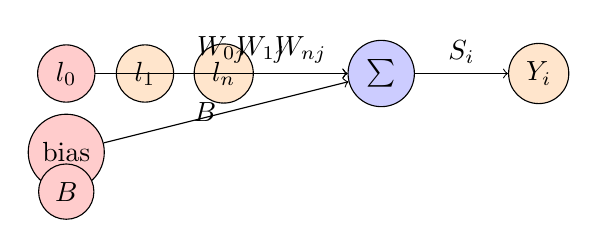
\begin{tikzpicture}
\node[draw, circle, fill=red!20] (input1) at (0,0) {$l_0$};
\node[draw, circle, fill=orange!20] (input2) at (1,0) {$l_1$};
\node[draw, circle, fill=orange!20] (input3) at (2,0) {$l_n$};
\node[draw, circle, fill=blue!20] (sum) at (4,0) {$\sum$};
\node[draw, circle, fill=orange!20] (output) at (6,0) {$Y_i$};
\node[draw, circle, fill=red!20] (bias) at (0,-1) {bias};
\node[draw, circle, fill=red!20] (bias_val) at (0,-1.5) {$B$};
\draw[->] (input1) -- (sum) node[midway, above] {$W_{0j}$};
\draw[->] (input2) -- (sum) node[midway, above] {$W_{1j}$};
\draw[->] (input3) -- (sum) node[midway, above] {$W_{nj}$};
\draw[->] (bias) -- (sum) node[midway, left] {$B$};
\draw[->] (sum) -- (output) node[midway, above] {$S_i$};
\end{tikzpicture}
\begin{itemize}
    \item Remind you of "logistic regression"?
\end{itemize}
\begin{tikzpicture}
\begin{axis}[
    xlabel={$z$},
    ylabel={$g(z)$},
    xmin=-8, xmax=8,
    ymin=0, ymax=1.1,
    title={Sigmoid},
]
\addplot[domain=-8:8, samples=100] {(1/(1+exp(-x)))};
\end{axis}
\end{tikzpicture}
\begin{tikzpicture}
\begin{axis}[
    xlabel={$z$},
    ylabel={$R(z)$},
    xmin=-8, xmax=8,
    ymin=0, ymax=8,
    title={ReLU},
]
\addplot[domain=-8:8, samples=100] {max(0,x)};
\end{axis}
\end{tikzpicture}
Jed Fox, "Neural Networks 101," 2017
%
\subsection{Description}%
This slide introduces the concept of an artificial neuron within the context of Artificial Intelligence Basics.  It visually depicts a multi-layered perceptron, showing the connections between input nodes (orange circles), a summation node (blue circle), and an output node (orange circle).  The input nodes represent the inputs to the neuron, and the weights (e.g., $W_{0j}$, $W_{1j}$, etc.) are associated with each connection.  The summation node ($\sum$) represents the weighted sum of the inputs.  The output node ($Y_i$) represents the output of the neuron, which is often passed through an activation function.  The bias ($B$) is a constant added to the weighted sum.  The slide also includes graphs of two common activation functions: the sigmoid function and the ReLU (Rectified Linear Unit) function.  The sigmoid function is a smooth, S-shaped curve that maps any input to a value between 0 and 1.  The ReLU function outputs the input if it's positive and 0 otherwise.  The slide also includes a reminder of logistic regression, suggesting a connection to previous material in the course.  The context of the course is focused on the fundamental building blocks of neural networks and their activation functions.%
\subsection{Figures}%
\begin{figure}[H]%
\centering%
\begin{subfigure}[b]{0.15\textwidth}%
\centering%

\includegraphics[width=\textwidth]{/Users/ashoksaravanan/Coding/ScribeLec/server/output/CS 243/lectures/09L1-cnn/figures/5.1.png}%
\caption{}%
\end{subfigure}%
\hspace{0.05\textwidth}%
\begin{subfigure}[b]{0.15\textwidth}%
\centering%

\includegraphics[width=\textwidth]{/Users/ashoksaravanan/Coding/ScribeLec/server/output/CS 243/lectures/09L1-cnn/figures/5.2.png}%
\caption{}%
\end{subfigure}%
\hspace{0.05\textwidth}%
\begin{subfigure}[b]{0.15\textwidth}%
\centering%

\includegraphics[width=\textwidth]{/Users/ashoksaravanan/Coding/ScribeLec/server/output/CS 243/lectures/09L1-cnn/figures/5.3.png}%
\caption{}%
\end{subfigure}%
\hspace{0.05\textwidth}%
\begin{subfigure}[b]{0.15\textwidth}%
\centering%

\includegraphics[width=\textwidth]{/Users/ashoksaravanan/Coding/ScribeLec/server/output/CS 243/lectures/09L1-cnn/figures/5.4.png}%
\caption{}%
\end{subfigure}%
\hspace{0.05\textwidth}%
\begin{subfigure}[b]{0.15\textwidth}%
\centering%

\includegraphics[width=\textwidth]{/Users/ashoksaravanan/Coding/ScribeLec/server/output/CS 243/lectures/09L1-cnn/figures/5.5.png}%
\caption{}%
\end{subfigure}%
\end{figure}

%
\newpage%
\section{Slide 6}%
\label{sec:Slide6}%
\subsection{Content}%

\textbf{Convolution and Pooling Layers} \\
Convolution layer \\
Optional pooling layer \\
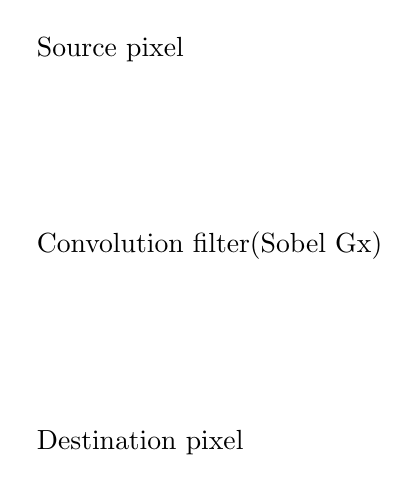
\begin{tikzpicture}
\node[anchor=west] at (0, 2.5) {Source pixel};
\node[anchor=west] at (0, 0) {Convolution filter \\ (Sobel Gx)};
\node[anchor=west] at (0, -2.5) {Destination pixel};
\end{tikzpicture}
\begin{tikzpicture}
\matrix[matrix of nodes, column sep=0.5cm, row sep=0.5cm] (matrix) {
2 & 0 & 0 & 3 & 0 \\
0 & 2 & 4 & 3 & 0 \\
0 & 0 & 6 & 2 & 0 \\
2 & 6 & 4 & 2 & 3 \\
0 & 0 & 2 & 0 & 0 \\
};
\end{tikzpicture}
\begin{tikzpicture}
\matrix[matrix of nodes, column sep=0.5cm, row sep=0.5cm] (matrix) {
31 & 7 & 44 & 33 \\
65 & 35 & 40 & 46 \\
46 & 29 & 32 & 30 \\
24 & 49 & 8 & 64 \\
};
\end{tikzpicture}
\begin{tikzpicture}
\matrix[matrix of nodes, column sep=0.5cm, row sep=0.5cm] (matrix) {
65 & 46 \\
46 & 64 \\
};
\end{tikzpicture}
\end{document}
%
\subsection{Description}%
This slide illustrates the convolution and pooling layers in a Convolutional Neural Network (CNN).  The left side shows a source pixel matrix (a 5x5 grid of numbers) and a convolution filter (Sobel Gx, likely a 3x3 matrix). The convolution operation is performed by sliding the filter across the source pixel matrix, performing element-wise multiplication and summation. The result of this operation is a destination pixel matrix (a 4x4 grid of numbers).  The right side shows the result of the convolution operation (31, 7, 44, 33, etc.) and then the result of a pooling operation (65, 46, 46, 64).  The slide visually depicts the process of extracting features from an image using convolution and then reducing the dimensionality using pooling.  The context of the course is focused on the fundamental building blocks of CNNs, crucial for understanding image recognition and processing tasks within Artificial Intelligence Basics.%
\subsection{Figures}%
\begin{figure}[H]%
\centering%
\begin{subfigure}[b]{0.15\textwidth}%
\centering%

\includegraphics[width=\textwidth]{/Users/ashoksaravanan/Coding/ScribeLec/server/output/CS 243/lectures/09L1-cnn/figures/6.1.png}%
\caption{}%
\end{subfigure}%
\end{figure}

%
\newpage%
\section{Slide 7}%
\label{sec:Slide7}%
\subsection{Content}%
%
\subsection{Description}%
This slide demonstrates a convolution operation in a Convolutional Neural Network (CNN).  A 3x3 convolution filter (matrix of numbers) is applied to a 5x5 input matrix (representing an image or feature map). The asterisk (*) symbol denotes the convolution operation. The result of the convolution is an output matrix (likely smaller than the input matrix). The slide shows the input and filter matrices, and the output matrix is partially shown, with the value 44 in the top-left cell and -1 in the top-right cell.  The slide also includes a calculation of the channel partial sum [0][0] which is equal to 44.  The text below the matrices indicates that zero padding is typically added to the input matrix to maintain the dimensions of the output matrix. The context of the course is Artificial Intelligence Basics, focusing on the fundamental operations within Convolutional Neural Networks, which are crucial for image processing and recognition tasks.%
\subsection{Figures}%
\begin{figure}[H]%
\centering%
\end{figure}

%
\newpage%
\section{Slide 8}%
\label{sec:Slide8}%
\subsection{Content}%

\textbf{Multidimensional Convolution} \\
"Feature Map" usually has multiple layers \\
\begin{itemize}
    \item An image has R, G, B layers, or "channels"
\end{itemize}
One layer has many convolution filters, which create a multichannel output map \\
\begin{tikzpicture}
\matrix[matrix of nodes, column sep=0.5cm, row sep=0.5cm] (matrix) {
\node[draw, fill=green!20] {}; & \node[draw, fill=orange!20] {}; \\
\node[draw, fill=green!20] {}; & \node[draw, fill=orange!20] {}; \\
};
\matrix[matrix of nodes, column sep=0.5cm, row sep=0.5cm, right=1cm of matrix] (matrix2) {
\node[draw, fill=blue!20] {1}; & \node[draw, fill=blue!20] {2}; & \node[draw, fill=blue!20] {3}; \\
\node[draw, fill=blue!20] {-2}; & \node[draw, fill=blue!20] {0}; & \node[draw, fill=blue!20] {-1}; \\
\node[draw, fill=blue!20] {5}; & \node[draw, fill=blue!20] {-2}; & \node[draw, fill=blue!20] {4}; \\
};
\node[right=0.5cm of matrix2] {$*$};
\matrix[matrix of nodes, column sep=0.5cm, row sep=0.5cm, right=1cm of matrix2] (matrix3) {
\node {}; & \node {}; \\
\node {}; & \node {}; \\
};
\node[below=0.5cm of matrix, text width=4cm] {Channels};
\node[below=0.5cm of matrix2, text width=4cm] {$3 \times 3 \times 3$ filter};
\node[below=0.5cm of matrix3, text width=4cm] {Output feature map};
\node[left=0.5cm of matrix] {Input feature map};
\node[right=0.5cm of matrix3] {$=$};
\end{tikzpicture}
\end{document}
%
\subsection{Description}%
This slide illustrates multidimensional convolution in a Convolutional Neural Network (CNN).  It shows how a 3x3x3 filter is applied to an input feature map with multiple channels (in this case, three). The input feature map is represented by three 3x3 matrices (green, orange, and light-red), each representing a different channel. The 3x3x3 filter is a 3x3 matrix with values (1, 2, 3; -2, 0, -1; 5, -2, 4) applied to each channel of the input feature map. The asterisk (*) symbol represents the convolution operation. The output feature map is a single 3x3 matrix, which is the result of applying the filter to each channel of the input feature map and combining the results. The slide emphasizes that a "Feature Map" typically has multiple layers, and an image can be represented by multiple channels (e.g., Red, Green, Blue in an RGB image). The context of the course is Artificial Intelligence Basics, focusing on the fundamental operations within Convolutional Neural Networks, which are crucial for image processing and recognition tasks.%
\subsection{Figures}%
\begin{figure}[H]%
\centering%
\end{figure}

%
\newpage%
\section{Slide 9}%
\label{sec:Slide9}%
\subsection{Content}%
%
\subsection{Description}%
This slide, part of a lecture on Artificial Intelligence Basics, illustrates the concept of multiple convolutions in a Convolutional Neural Network (CNN).  It shows how multiple filters are applied to an input feature map.  The input feature map is a grid of cells (represented by a matrix of nodes).  Multiple filters (Filter 0 and Filter 1, in this case, depicted by stacked grids of the same size as the input feature map) are applied to the input feature map.  The application of each filter results in an output feature map (Output feature map 0 and Output feature map 1).  The output feature maps are also grids of cells, the same size as the input feature map.  The slide visually demonstrates how different filters extract different features from the input image, creating multiple feature maps that are then used in subsequent layers of the network.  The context of the course is focused on the fundamental building blocks of CNNs, crucial for understanding image recognition and processing tasks within Artificial Intelligence Basics.%
\subsection{Figures}%
\begin{figure}[H]%
\centering%
\end{figure}

%
\newpage%
\section{Slide 10}%
\label{sec:Slide10}%
\subsection{Content}%
%
\subsection{Description}%
This slide, part of a lecture on Artificial Intelligence Basics, discusses why convolutional neural networks (CNNs) use convolution instead of fully connected layers.  It visually contrasts sparse connectivity in a CNN with dense connectivity in a standard neural network.  The top portion of the slide shows a diagram of a convolutional layer.  Nodes $x_1$ through $x_{15}$ represent input features (likely from an image).  Connections between these nodes are sparse, meaning each node in the convolutional layer is only connected to a small neighborhood of input nodes (defined by the convolution kernel).  This is labeled "Sparse connections due to small convolution kernel."  The bottom portion of the slide shows a diagram of a fully connected layer.  Here, every node in the layer is connected to every input node.  This is labeled "Dense connections."  The visual difference highlights that convolution significantly reduces the number of parameters compared to a fully connected layer, making CNNs more efficient for processing image data.  The context of the course is focused on the fundamental building blocks of CNNs, explaining why convolution is a key concept in image recognition and processing tasks within Artificial Intelligence Basics.%
\subsection{Figures}%
\begin{figure}[H]%
\centering%
\begin{subfigure}[b]{0.15\textwidth}%
\centering%

\includegraphics[width=\textwidth]{/Users/ashoksaravanan/Coding/ScribeLec/server/output/CS 243/lectures/09L1-cnn/figures/10.1.png}%
\caption{}%
\end{subfigure}%
\end{figure}

%
\newpage%
\section{Slide 11}%
\label{sec:Slide11}%
\subsection{Content}%

\textbf{Why convolution? Not fully connected?} \\
Sparse connectivity: being affected by less \\
\begin{tikzpicture}
\matrix[matrix of nodes, column sep=0.5cm, row sep=0.5cm] (matrix) {
\node {$x_1$}; & \node {$x_2$}; & \node {$x_3$}; & \node {$x_4$}; & \node {$x_5$}; \\
\node {$x_{21}$}; & \node {$x_{22}$}; & \node {$x_{23}$}; & \node {$x_{24}$}; & \node {$x_{25}$}; \\
};
\foreach \i in {1,2,3,4,5}
\draw[->] (matrix-1-\i) -- (matrix-2-\i);
\foreach \i in {1,2,3,4,5}
\draw[->] (matrix-1-\i) -- (matrix-2-\i);
\foreach \i in {1,2,3,4,5}
\draw[->] (matrix-1-\i) -- (matrix-2-\i);
\foreach \i in {1,2,3,4,5}
\draw[->] (matrix-1-\i) -- (matrix-2-\i);
\foreach \i in {1,2,3,4,5}
\draw[->] (matrix-1-\i) -- (matrix-2-\i);
\node[below=0.5cm of matrix] {Sparse connections \\ due to small \\ convolution kernel};
\end{tikzpicture}
\begin{tikzpicture}[xscale=1.5]
\matrix[matrix of nodes, column sep=0.5cm, row sep=0.5cm] (matrix2) {
\node {$x_1$}; & \node {$x_2$}; & \node {$x_3$}; & \node {$x_4$}; & \node {$x_5$}; \\
\node {$x_{21}$}; & \node {$x_{22}$}; & \node {$x_{23}$}; & \node {$x_{24}$}; & \node {$x_{25}$}; \\
};
\foreach \i in {1,2,3,4,5}
\foreach \j in {1,2,3,4,5}
\draw[->] (matrix2-1-\i) -- (matrix2-2-\j);
\node[below=0.5cm of matrix2] {Dense connections};
\end{tikzpicture}
\end{LATEX}
%
\subsection{Description}%
This slide from an Artificial Intelligence Basics course explains why convolutional neural networks (CNNs) use convolution instead of fully connected layers.  It visually contrasts the sparse connectivity of a convolutional layer with the dense connectivity of a standard neural network.  The top diagram depicts a convolutional layer, where each node in the layer is connected to a small neighborhood of input nodes (defined by the convolution kernel).  This is labeled "Sparse connections due to small convolution kernel."  The bottom diagram shows a fully connected layer, where every node in the layer is connected to every input node.  This is labeled "Dense connections."  The visual difference highlights that convolution significantly reduces the number of parameters compared to a fully connected layer, making CNNs more efficient for processing image data.  The context of the course is focused on the fundamental building blocks of CNNs, explaining why convolution is a key concept in image recognition and processing tasks.%
\subsection{Figures}%
\begin{figure}[H]%
\centering%
\begin{subfigure}[b]{0.15\textwidth}%
\centering%

\includegraphics[width=\textwidth]{/Users/ashoksaravanan/Coding/ScribeLec/server/output/CS 243/lectures/09L1-cnn/figures/11.1.png}%
\caption{}%
\end{subfigure}%
\end{figure}

%
\newpage%
\section{Slide 12}%
\label{sec:Slide12}%
\subsection{Content}%
%
\subsection{Description}%
This slide from an Artificial Intelligence Basics course discusses the difference in parameter sharing between convolutional and traditional matrix multiplication in neural networks.  The top portion of the slide shows a diagram of a convolutional layer.  The nodes $s_1$ through $s_5$ represent input parameters, and the nodes $x_1$ through $x_5$ represent output parameters.  The connections between these nodes are shown as gray arrows.  The text "Convolution shares the same parameters across all spatial locations" highlights the key characteristic of convolution: the same parameters ($s_i$) are used for different spatial locations in the input.  The bottom portion of the slide shows a diagram of a traditional matrix multiplication layer.  Here, each node in the output layer is connected to every node in the input layer.  The text "Traditional matrix multiplication does not share any parameters" emphasizes that each connection has a unique parameter.  The visual difference highlights that convolution significantly reduces the number of parameters compared to a fully connected layer, making CNNs more efficient for processing image data.  The context of the course is focused on the fundamental building blocks of CNNs, explaining why convolution is a key concept in image recognition and processing tasks.%
\subsection{Figures}%
\begin{figure}[H]%
\centering%
\begin{subfigure}[b]{0.15\textwidth}%
\centering%

\includegraphics[width=\textwidth]{/Users/ashoksaravanan/Coding/ScribeLec/server/output/CS 243/lectures/09L1-cnn/figures/12.1.png}%
\caption{}%
\end{subfigure}%
\end{figure}

%
\newpage%
\section{Slide 13}%
\label{sec:Slide13}%
\subsection{Content}%
%
\subsection{Description}%
This slide from an Artificial Intelligence Basics course introduces the Rectified Linear Unit (ReLU) activation function.  It displays the graph of the ReLU function, which is defined as $f(u) = \max(0, u)$.  The graph shows a straight line starting at the origin (0,0) and extending upward with a slope of 1 for $u \ge 0$.  For $u < 0$, the function outputs 0.  The horizontal axis is labeled $u$, and the vertical axis is labeled $f(u)$.  The graph clearly illustrates the piecewise linear nature of the ReLU function.  The title and the equation $f(x) = \max(0, x)$ further define the function. The context of the course is focused on activation functions used in neural networks, explaining how ReLU functions introduce non-linearity into the network's behavior.%
\subsection{Figures}%
\begin{figure}[H]%
\centering%
\begin{subfigure}[b]{0.15\textwidth}%
\centering%

\includegraphics[width=\textwidth]{/Users/ashoksaravanan/Coding/ScribeLec/server/output/CS 243/lectures/09L1-cnn/figures/13.1.png}%
\caption{}%
\end{subfigure}%
\end{figure}

%
\newpage%
\section{Slide 14}%
\label{sec:Slide14}%
\subsection{Content}%
%
\subsection{Description}%
This slide from an Artificial Intelligence Basics course explains the pooling layer in convolutional neural networks (CNNs).  The top part of the slide shows a diagram illustrating the spatial downsampling of an input volume.  A 224x224x64 input volume is downsampled to a 112x112x64 output volume.  The process is depicted as a "pool" operation.  The bottom part of the slide shows a single depth slice of the input volume and the corresponding output after the pooling operation.  The input slice is a 112x112 matrix of numbers.  The output slice is a 56x56 matrix of numbers.  The pooling operation, in this case, is max pooling with a 2x2 filter and a stride of 2.  The operation selects the maximum value within each 2x2 block of the input and places it in the corresponding output location.  The text describes that the pooling layer downsamples the input volume spatially, independently in each depth slice.  The example shows that the volume depth is preserved, and the most common downsampling operation is max pooling.  The context of the course is focused on the fundamental building blocks of CNNs, explaining how pooling layers reduce the spatial dimensions of feature maps while retaining important information.%
\subsection{Figures}%
\begin{figure}[H]%
\centering%
\begin{subfigure}[b]{0.15\textwidth}%
\centering%

\includegraphics[width=\textwidth]{/Users/ashoksaravanan/Coding/ScribeLec/server/output/CS 243/lectures/09L1-cnn/figures/14.1.png}%
\caption{}%
\end{subfigure}%
\end{figure}

%
\newpage%
\section{Slide 15}%
\label{sec:Slide15}%
\subsection{Content}%

\begin{tikzpicture}
\matrix[matrix of nodes,ampersand replacement=\&,column sep=0.5cm,row sep=0.5cm] {
\& \node[draw,rectangle,red] {12}; \& \node[draw,rectangle,red] {20}; \& \node[draw,rectangle,red] {30}; \& \node[draw,rectangle,red] {0}; \\
\& \node[draw,rectangle,blue] {8}; \& \node[draw,rectangle,blue] {12}; \& \node[draw,rectangle,blue] {2}; \& \node[draw,rectangle,blue] {0}; \\
\& \node[draw,rectangle,green] {34}; \& \node[draw,rectangle,green] {70}; \& \node[draw,rectangle,green] {37}; \& \node[draw,rectangle,green] {4}; \\
\& \node[draw,rectangle,yellow] {112}; \& \node[draw,rectangle,yellow] {100}; \& \node[draw,rectangle,yellow] {25}; \& \node[draw,rectangle,yellow] {12}; \\
};
\draw[->,>=latex] (2.5,3.5) -- (5.5,5.5) node[midway,above] {max pooling};
\draw[->,>=latex] (2.5,3.5) -- (8.5,3.5) node[midway,below] {average pooling};
\matrix[matrix of nodes,ampersand replacement=\&,column sep=0.5cm,row sep=0.5cm,right=2cm of current bounding box] {
\& \node[draw,rectangle] {20}; \& \node[draw,rectangle] {30}; \\
\& \node[draw,rectangle] {112}; \& \node[draw,rectangle] {37}; \\
};
\matrix[matrix of nodes,ampersand replacement=\&,column sep=0.5cm,row sep=0.5cm,below=1cm of current bounding box] {
\& \node[draw,rectangle] {13}; \& \node[draw,rectangle] {8}; \\
\& \node[draw,rectangle] {79}; \& \node[draw,rectangle] {20}; \\
};
\end{tikzpicture}
%
\subsection{Description}%
This slide from an Artificial Intelligence Basics course demonstrates the pooling operation in convolutional neural networks (CNNs).  It shows two types of pooling: max pooling and average pooling.  The input is a 4x4 matrix of numbers.  Max pooling selects the maximum value within each 2x2 block of the input matrix and places it in the corresponding output location.  In the example, the maximum value in the top-left 2x2 block is 20, and the maximum value in the top-right 2x2 block is 30.  The output of max pooling is a 2x2 matrix.  Average pooling calculates the average of the values within each 2x2 block and places it in the corresponding output location.  In the example, the average of the values in the top-left 2x2 block is 13, and the average of the values in the top-right 2x2 block is 8.  The output of average pooling is also a 2x2 matrix.  The slide visually illustrates the process of downsampling feature maps in CNNs, which reduces computational cost and helps to extract important features. The context of the course is focused on the fundamental building blocks of CNNs, explaining how pooling layers reduce the spatial dimensions of feature maps while retaining important information.%
\subsection{Figures}%
\begin{figure}[H]%
\centering%
\begin{subfigure}[b]{0.15\textwidth}%
\centering%

\includegraphics[width=\textwidth]{/Users/ashoksaravanan/Coding/ScribeLec/server/output/CS 243/lectures/09L1-cnn/figures/15.1.png}%
\caption{}%
\end{subfigure}%
\end{figure}

%
\newpage%
\section{Slide 16}%
\label{sec:Slide16}%
\subsection{Content}%
%
\subsection{Description}%
%
\subsection{Figures}%
\begin{figure}[H]%
\centering%
\begin{subfigure}[b]{0.15\textwidth}%
\centering%

\includegraphics[width=\textwidth]{/Users/ashoksaravanan/Coding/ScribeLec/server/output/CS 243/lectures/09L1-cnn/figures/16.1.png}%
\caption{}%
\end{subfigure}%
\end{figure}

%
\newpage%
\section{Slide 17}%
\label{sec:Slide17}%
\subsection{Content}%
%
\subsection{Description}%
This slide from an Artificial Intelligence Basics course presents a diagram of a simple Convolutional Neural Network (CNN) structure.  The diagram visually depicts the sequential layers of a CNN, starting with the input image (a picture of a Tesla car).  The layers are labeled with their respective functions:

* **CONV:** Convolutional kernel layer: This layer applies filters (kernels) to the input image to extract features.  The diagram shows multiple CONV layers, indicating multiple feature extraction stages.  The output of each CONV layer is a set of feature maps.

* **RELU:** Rectified Linear Unit activation function: This layer introduces non-linearity to the network.  The diagram shows multiple RELU layers, suggesting that the non-linearity is applied after each convolution operation.

* **POOL:** Dimension reduction layer: This layer reduces the spatial dimensions of the feature maps, typically using max-pooling or average-pooling.  The diagram shows multiple POOL layers, indicating that the spatial dimensions are reduced multiple times.

* **FC:** Fully connected layer: This layer connects all the features extracted from the previous layers to produce the final output.  The diagram shows a single FC layer at the end of the network.

The diagram also shows the output classes (e.g., car, truck, airplane, ship, horse) that the CNN is trained to recognize.  The output classes are shown in a list below the FC layer.  The context of the course is focused on the fundamental building blocks of CNNs, illustrating how these layers work together to process images and classify them into different categories.%
\subsection{Figures}%
\begin{figure}[H]%
\centering%
\begin{subfigure}[b]{0.15\textwidth}%
\centering%

\includegraphics[width=\textwidth]{/Users/ashoksaravanan/Coding/ScribeLec/server/output/CS 243/lectures/09L1-cnn/figures/17.1.png}%
\caption{}%
\end{subfigure}%
\end{figure}

%
\newpage%
\section{Slide 18}%
\label{sec:Slide18}%
\subsection{Content}%
%
\subsection{Description}%
This slide displays a grid of learned convolutional filters.  Each small square within the grid represents a filter learned by a Convolutional Neural Network (CNN) during training.  The filters are likely learned to detect various visual patterns in images.  The colors and patterns within the filters vary, indicating the different types of features the filters are designed to recognize.  The title "Example Learned Convolution Filters" clearly identifies the content of the slide.  The attribution "Alex Krizhevsky et al., "ImageNet Classification with Deep Convolutional Neural Networks," NIPS, 2012" indicates the source of the filters and the context of the research paper, which likely details the training process and the purpose of these filters within a larger image classification task.  The context of the course (Artificial Intelligence Basics) suggests that the slide is illustrating a key component of CNNs, specifically how they learn to extract relevant features from images.%
\subsection{Figures}%
\begin{figure}[H]%
\centering%
\begin{subfigure}[b]{0.15\textwidth}%
\centering%

\includegraphics[width=\textwidth]{/Users/ashoksaravanan/Coding/ScribeLec/server/output/CS 243/lectures/09L1-cnn/figures/18.1.png}%
\caption{}%
\end{subfigure}%
\end{figure}

%
\newpage%
\section{Slide 19}%
\label{sec:Slide19}%
\subsection{Content}%
%
\subsection{Description}%
This slide from an Artificial Intelligence Basics course illustrates the concept of multidimensional convolution in a Convolutional Neural Network (CNN).  A grayscale image of a city skyline is shown as the input image.  A set of smaller, grayscale filters (a "filter bank") is applied to a portion of the input image.  The result of applying each filter is a feature map.  The feature maps are shown as a result of applying the filter bank to the input image.  The filters are to be learned during the training process of the CNN.  The slide visually demonstrates how the filters extract features from the input image, transforming it into feature maps.  The context of the course is focused on the fundamental building blocks of CNNs, illustrating how these layers work together to process images and extract relevant information.%
\subsection{Figures}%
\begin{figure}[H]%
\centering%
\begin{subfigure}[b]{0.15\textwidth}%
\centering%

\includegraphics[width=\textwidth]{/Users/ashoksaravanan/Coding/ScribeLec/server/output/CS 243/lectures/09L1-cnn/figures/19.1.png}%
\caption{}%
\end{subfigure}%
\end{figure}

%
\newpage%
\section{Slide 20}%
\label{sec:Slide20}%
\subsection{Content}%

\textbf{Biology Inspiration}

\begin{figure}[h]
\centering
\includegraphics[width=0.4\textwidth]{biological_brain_diagram.png}
\caption{FIG. 1 - Organization of a biological brain. (Red areas indicate active cells, responding to the letter X.)}
\end{figure}

\begin{figure}[h]
\centering
\includegraphics[width=0.4\textwidth]{perceptron_diagram.png}
\caption{FIG. 2 - Organization of a perceptron.}
\end{figure}

\end{document}
%
\subsection{Description}%
This slide, part of an Artificial Intelligence Basics course, presents a biological inspiration for artificial neural networks.  It features two diagrams:

**FIG. 1:**  Illustrates the organization of a biological brain.  Red areas represent active cells responding to a stimulus (likely a visual input, like the letter "X").  The diagram shows sensory input, projection areas, and an association system.  Arrows indicate the direction of signal flow.  The diagram highlights the concept of topographic connections (connections between cells in a specific spatial arrangement) and random connections.  The diagram also shows feedback circuits.

**FIG. 2:**  Depicts the organization of a perceptron, a fundamental unit in artificial neural networks.  The diagram shows inputs ($l_0$, $l_n$), weights ($w_{0j}$, $w_{1j}$, $w_{nj}$), a bias ($B$), and a summation ($\sum$).  The output ($Y$) is calculated based on the weighted sum of inputs plus the bias.  A sigmoid function (represented by the curved line) is applied to the result of the summation.  The diagram visually represents the mathematical function of a perceptron: $Y = \sigma(\sum_{i=0}^{n} w_{ij} l_i + B)$, where $\sigma$ is the sigmoid function.

The slide uses biological neural networks as a conceptual model for artificial neural networks, highlighting the similarities in signal processing and information flow.  The context of the course is focused on the fundamental building blocks of artificial neural networks and their biological inspiration.  The URL at the bottom of the slide likely links to further details about the neural networks project.%
\subsection{Figures}%
\begin{figure}[H]%
\centering%
\begin{subfigure}[b]{0.15\textwidth}%
\centering%

\includegraphics[width=\textwidth]{/Users/ashoksaravanan/Coding/ScribeLec/server/output/CS 243/lectures/09L1-cnn/figures/20.1.png}%
\caption{}%
\end{subfigure}%
\hspace{0.05\textwidth}%
\begin{subfigure}[b]{0.15\textwidth}%
\centering%

\includegraphics[width=\textwidth]{/Users/ashoksaravanan/Coding/ScribeLec/server/output/CS 243/lectures/09L1-cnn/figures/20.2.png}%
\caption{}%
\end{subfigure}%
\hspace{0.05\textwidth}%
\begin{subfigure}[b]{0.15\textwidth}%
\centering%

\includegraphics[width=\textwidth]{/Users/ashoksaravanan/Coding/ScribeLec/server/output/CS 243/lectures/09L1-cnn/figures/20.3.png}%
\caption{}%
\end{subfigure}%
\end{figure}

%
\newpage%
\section{Slide 21}%
\label{sec:Slide21}%
\subsection{Content}%

\textbf{MNIST dataset of handwritten digits}

A training set of 60,000 examples \\
A test set of 10,000 examples. \\
A larger set is available from NIST. \\
The digits have been size-normalized and \\
centered in a fixed-size image.

\end{document}
%
\subsection{Description}%
This slide, part of an Artificial Intelligence Basics course, introduces the MNIST dataset.  It states that the dataset contains handwritten digits.  A training set of 60,000 examples and a test set of 10,000 examples are provided.  The slide also mentions that a larger dataset is available from NIST (National Institute of Standards and Technology).  Crucially, the slide highlights that the digits in the MNIST dataset have been preprocessed: they are size-normalized and centered within a fixed-size image.  This preprocessing step is important for ensuring consistency and efficiency in training machine learning models on the data.  The slide likely precedes a discussion of using this dataset for image recognition tasks, such as digit classification.%
\subsection{Figures}%
\begin{figure}[H]%
\centering%
\begin{subfigure}[b]{0.15\textwidth}%
\centering%

\includegraphics[width=\textwidth]{/Users/ashoksaravanan/Coding/ScribeLec/server/output/CS 243/lectures/09L1-cnn/figures/21.1.png}%
\caption{}%
\end{subfigure}%
\end{figure}

%
\newpage%
\section{Slide 22}%
\label{sec:Slide22}%
\subsection{Content}%

\textbf{LeNet-5 for MNIST}

\begin{itemize}
    \item \textbf{Input}: $28 \times 28 \times 1$
    \item Conv: $5 \times 5$, 32 filters, Padding: 2
    \item Pool: $2 \times 2$, stride: 2
    \item Conv: $5 \times 5$, 64 filters, Padding: 2
    \item Pool: $2 \times 2$, stride: 2
    \item Flatten features $\rightarrow$ $1 \times 1 \times 1024$
    \item Fc 1,2, 1024
    \item Dropout 0.5
    \item \textbf{Output}: $1 \times 1 \times 10$
\end{itemize}

\end{document}
%
\subsection{Description}%
This slide, part of an Artificial Intelligence Basics course, details the architecture of LeNet-5, a convolutional neural network (CNN) designed for the MNIST handwritten digit recognition task.  The diagram visually represents the layers of the network, showing the input image size (28x28x1), followed by convolutional layers (Conv), pooling layers (Pool), and finally a fully connected layer (Fc) leading to the output.  Each convolutional layer is described with its kernel size (5x5), the number of filters used (32 and 64), and padding (2).  The pooling layers use a 2x2 pooling window with a stride of 2.  The final layer flattens the feature maps into a single vector (1x1x1024) before passing it through a fully connected layer (Fc) with 1024 neurons, followed by a dropout layer with a rate of 0.5, and finally an output layer (1x1x10) that produces a probability distribution over the 10 possible digits (0-9).  The slide visually illustrates the flow of data through the network, highlighting the progressive dimensionality reduction and feature extraction steps characteristic of CNNs.  The context of the course is focused on the practical application of CNNs for image recognition tasks.%
\subsection{Figures}%
\begin{figure}[H]%
\centering%
\begin{subfigure}[b]{0.15\textwidth}%
\centering%

\includegraphics[width=\textwidth]{/Users/ashoksaravanan/Coding/ScribeLec/server/output/CS 243/lectures/09L1-cnn/figures/22.1.png}%
\caption{}%
\end{subfigure}%
\end{figure}

%
\newpage%
\section{Slide 23}%
\label{sec:Slide23}%
\subsection{Content}%
%
\subsection{Description}%
This slide presents the CIFAR-10 dataset, a benchmark dataset commonly used in image classification tasks.  It's part of an Artificial Intelligence Basics course.  The slide details the dataset's characteristics: 60,000 32x32 color images categorized into 10 classes (airplane, automobile, bird, cat, deer, dog, frog, horse, ship, truck).  Each class contains 6000 images.  The dataset is split into 50,000 training images and 10,000 test images.  The slide also includes a table showcasing the accuracy achieved by various state-of-the-art models (VGG16, ResNet18, ResNet50, ResNet101, ResNeXt29, DenseNet121, PreActResNet18, and DPN92) on the CIFAR-10 dataset.  The table lists each model and its corresponding accuracy percentage.  The visual representation of the dataset (images of different categories) and the table of accuracy scores provide a comprehensive overview of the CIFAR-10 dataset and its performance metrics for different models.  The context of the course suggests a discussion of image classification, deep learning models, and evaluating their performance on standard datasets.%
\subsection{Figures}%
\begin{figure}[H]%
\centering%
\begin{subfigure}[b]{0.15\textwidth}%
\centering%

\includegraphics[width=\textwidth]{/Users/ashoksaravanan/Coding/ScribeLec/server/output/CS 243/lectures/09L1-cnn/figures/23.1.png}%
\caption{}%
\end{subfigure}%
\hspace{0.05\textwidth}%
\begin{subfigure}[b]{0.15\textwidth}%
\centering%

\includegraphics[width=\textwidth]{/Users/ashoksaravanan/Coding/ScribeLec/server/output/CS 243/lectures/09L1-cnn/figures/23.2.png}%
\caption{}%
\end{subfigure}%
\end{figure}

%
\newpage%
\end{document}